\chapter{\IfLanguageName{dutch}{Over de metingen}{About the measurements}}
\label{ch:metingen}

\section{De gebruikstijd bij bepaalde opdrachten}
\label{sec:gebruikstijd}

Eén van de gemeten variabelen was de gebruikstijd bij bepaalde opdrachten. Er werd gemeten hoe lang de participant erover deed om bepaalde opdrachten te voltooien. De opdrachten waren bij alle participanten gelijk:
\begin{enumerate}
    \item Enkele instellingen wijzigen
    \item Een nieuw spaardoel toevoegen
    \item Een bedrag toevoegen aan een spaardoel
    \item Een reeds voltooid spaardoel verwijderen
    \item Een berekening met de ingebouwde calculator
    \item Een groot bedrag toevoegen aan een spaardoel
\end{enumerate}

De laatste opdracht werd pas na een korte onderbreking uitgevoerd. Deze opdracht is in essentie een herhaling van opdracht 3 (een bedrag toevoegen aan een spaardoel). Door deze achteraf nog eens uit te voeren werd getest of de participant de werking van die functionaliteit nog steeds onder de knie had.

De timer werd gepauzeerd wanneer de participant doorheen de onboarding ging. Ook wanneer er een help-element tevoorschijn kwam werd deze timer even stopgezet. Participanten kregen geen hulp van de moderator. De timer werd stopgezet nadat de participant voltooid had of wanneer de participant na een hele poos zijn of haar zoektocht opgaf.

In tabellen~\ref{tab:beschrijving-tijden-zonder-elementen} en \ref{tab:beschrijving-tijden-met-elementen} worden de gemiddelden en standaardafwijkingen van de gemeten tijden weergegeven. Hier kan men waarnemen dat er eventueel een verschil zal zijn in tijden tussen de groep die de opdrachten zonder onboarding en help-elementen voltooiden en de groep die de opdrachten met voltooiden. Het verschil wordt in hoofdstuk~\ref{sec:onderzoeksvraag-1} bewezen.

\begin{table}[]
	\centering
	\begin{tabular}{r|ccccccc}
		\multicolumn{1}{l|}{} & \multicolumn{7}{c}{\textit{Tijd in seconden}} \\
		& $Min$ & $Q_1$ & $Mdn$ & $M$ & $SD$ & $Q_3$ & $Max$ \\ \hline
		Instellingen & 7.00 & 15.00 & 19.50 & 24.08 & 12.87 & 31.25 & 45.00 \\
		Spaardoel toevoegen & 27.00 & 39.00 & 42.50 & 48.83 & 20.70 & 52.50 & 106.00 \\
		Bedrag toevoegen & 12.00 & 24.50 & 30.00 & 35.67 & 18.52 & 44.00 & 71.00 \\
		Spaardoel verwijderen & 11.00 & 14.25 & 39.50 & 65.25 & 57.46 & 121.50 & 148.00 \\
		Berekening & 22.00 & 34.75 & 38.00 & 40.33 & 17.5 & 41.50 & 91.00 \\
		Groot bedrag toevoegen & 12.00 & 25.50 & 34.00 & 47.25 & 35.76 & 50.75 & 137.00
	\end{tabular}
	\caption{Beschrijving van tijden zonder het gebruik van onboarding en help-elementen}
	\label{tab:beschrijving-tijden-zonder-elementen}
\end{table}

\begin{table}[]
	\centering
	\begin{tabular}{r|ccccccc}
		\multicolumn{1}{l|}{} & \multicolumn{7}{c}{\textit{Tijd in seconden}} \\
		& $Min$ & $Q_1$ & $Mdn$ & $M$ & $SD$ & $Q_3$ & $Max$ \\ \hline
		Instellingen & 5.00 & 12.00 & 15.00 & 15.31 & 7.39 & 15.00 & 30.00 \\
		Spaardoel toevoegen & 23.00 & 26.00 & 31.00 & 34.92 & 13.77 & 40.00 & 75.00 \\
		Bedrag toevoegen & 15.00 & 16.00 & 20.00 & 22.62 & 8.03 & 30.00 & 40.00 \\
		Spaardoel verwijderen & 6.00 & 8.00 & 15.00 & 16.38 & 11.94 & 20.00 & 48.00 \\
		Berekening & 12.00 & 20.00 & 25.00 & 26.15 & 9.33 & 30.00 & 42.00 \\
		Groot bedrag toevoegen & 10.00 & 12.00 & 17.00 & 24.77 & 27.88 & 26.00 & 115.00
	\end{tabular}
	\caption{Beschrijving van tijden met het gebruik van onboarding en help-elementen}
	\label{tab:beschrijving-tijden-met-elementen}
\end{table}

\section{Het vragen om hulp}
\label{sec:vragen-hulp}

Niet elke participant kon elke opdracht succesvol voltooien. In figuur~\ref{fig:beschrijving-hulp} wordt procentueel weergegeven indien men hulp nodig had bij het voltooien van de opdrachten. Er wordt een onderverdeling gemaakt indien men al dan niet gebruik kon maken van onboarding en help-elementen.

\begin{figure}[h]
    \centering
    \subfloat[Instellingen]{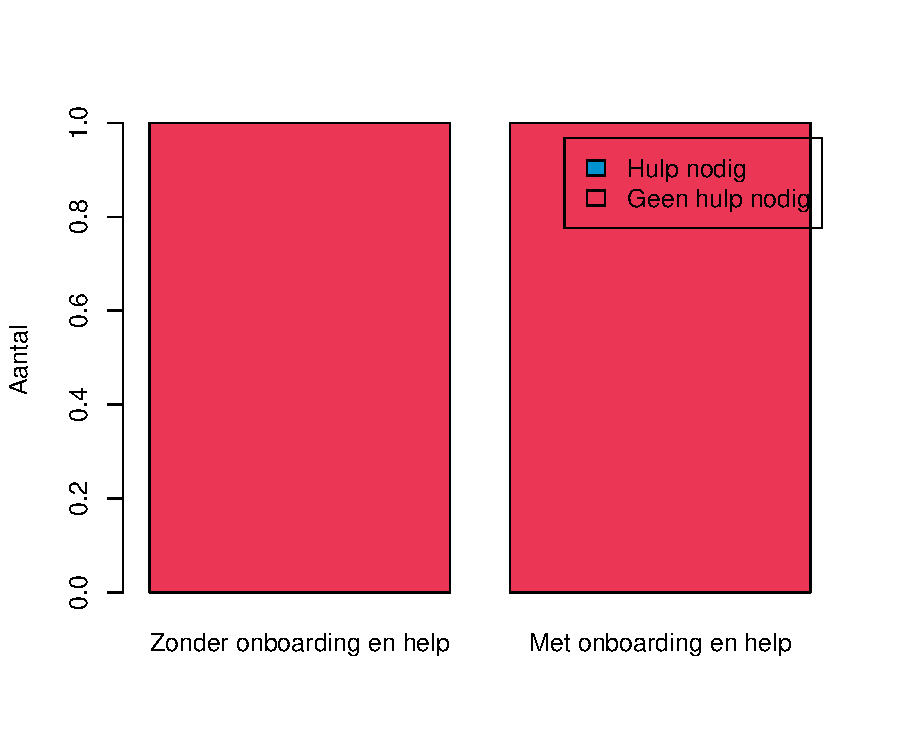
\includegraphics[width=.46\columnwidth]{beschrijving-hulp-instellingen}}
    \qquad
    \subfloat[Spaardoel toevoegen]{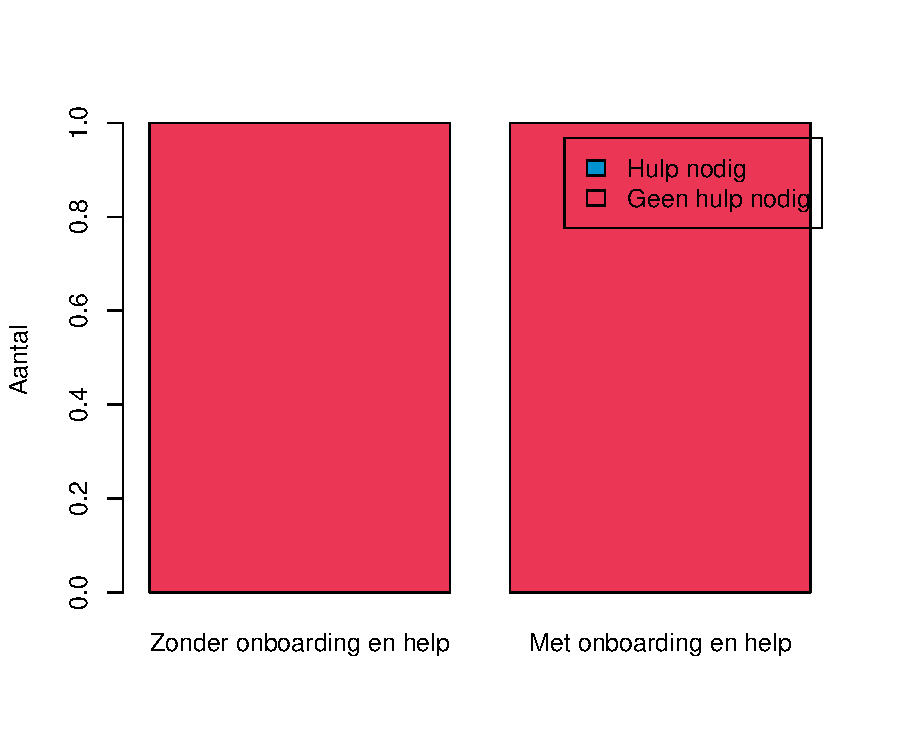
\includegraphics[width=.46\columnwidth]{beschrijving-hulp-spaardoel-toevoegen}}
    \qquad
    \subfloat[Bedrag toevoegen]{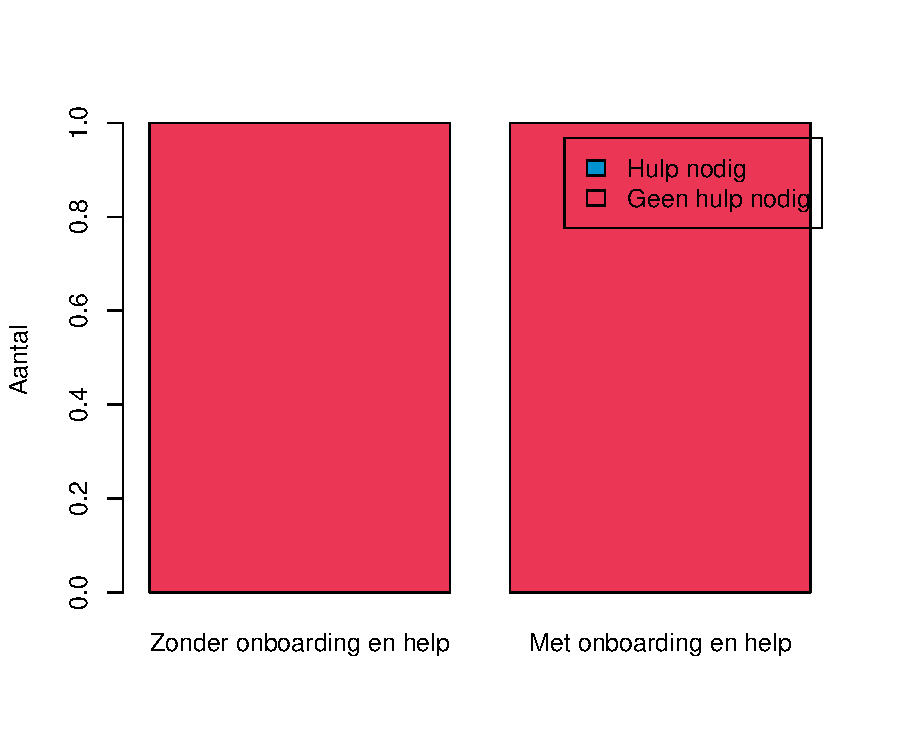
\includegraphics[width=.46\columnwidth]{beschrijving-hulp-bedrag-toevoegen}}
    \qquad
    \subfloat[Spaardoel verwijderen]{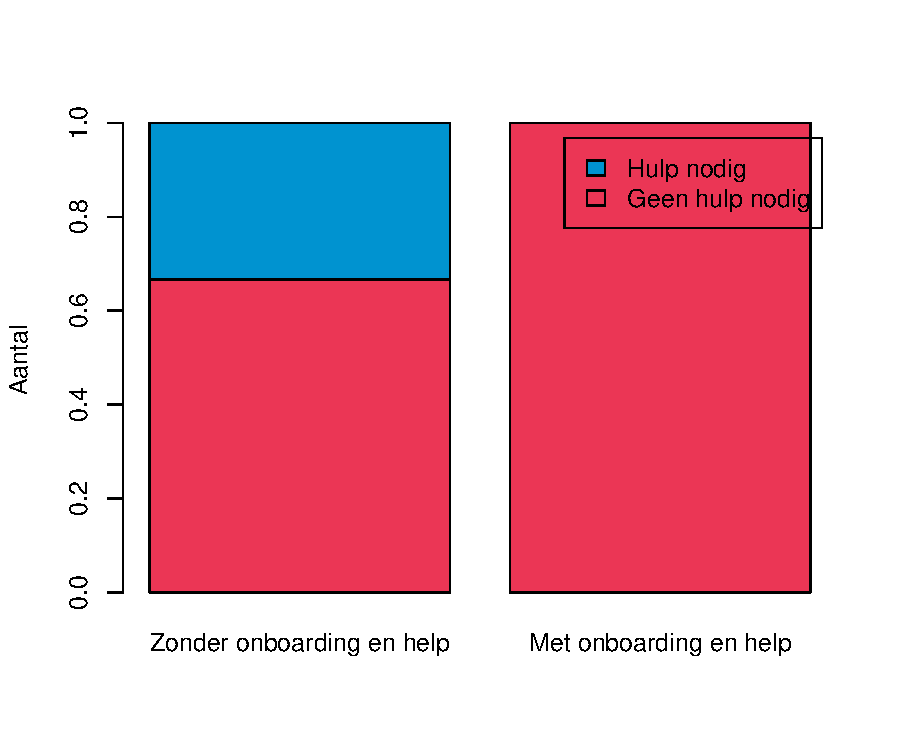
\includegraphics[width=.46\columnwidth]{beschrijving-hulp-spaardoel-verwijderen}}
    \qquad
    \subfloat[Berekening]{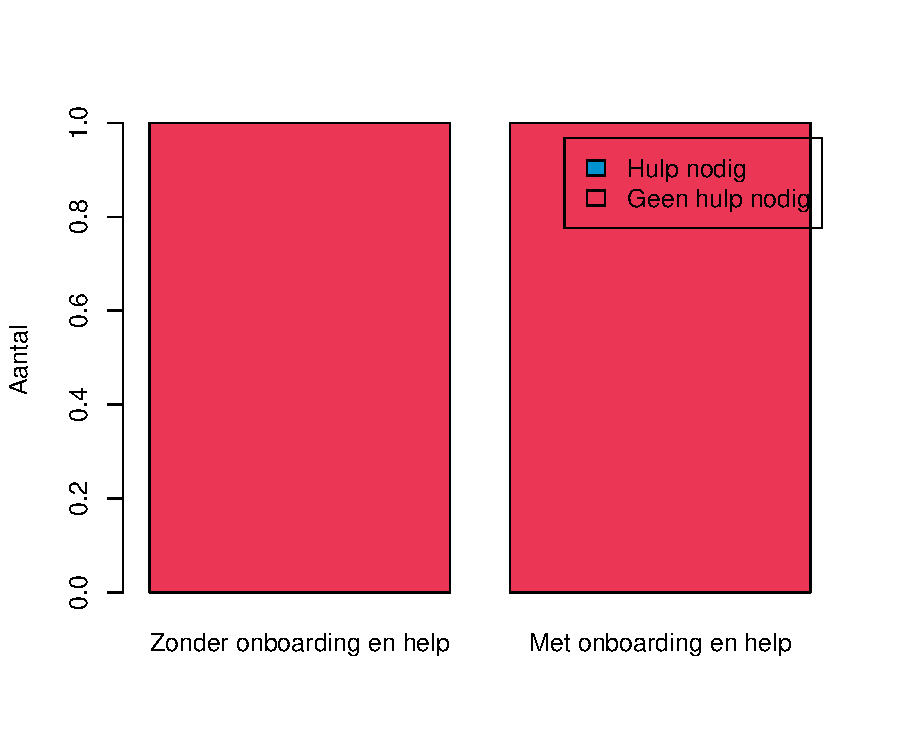
\includegraphics[width=.46\columnwidth]{beschrijving-hulp-berekening}}
    \qquad
    \subfloat[Groot bedrag toevoegen]{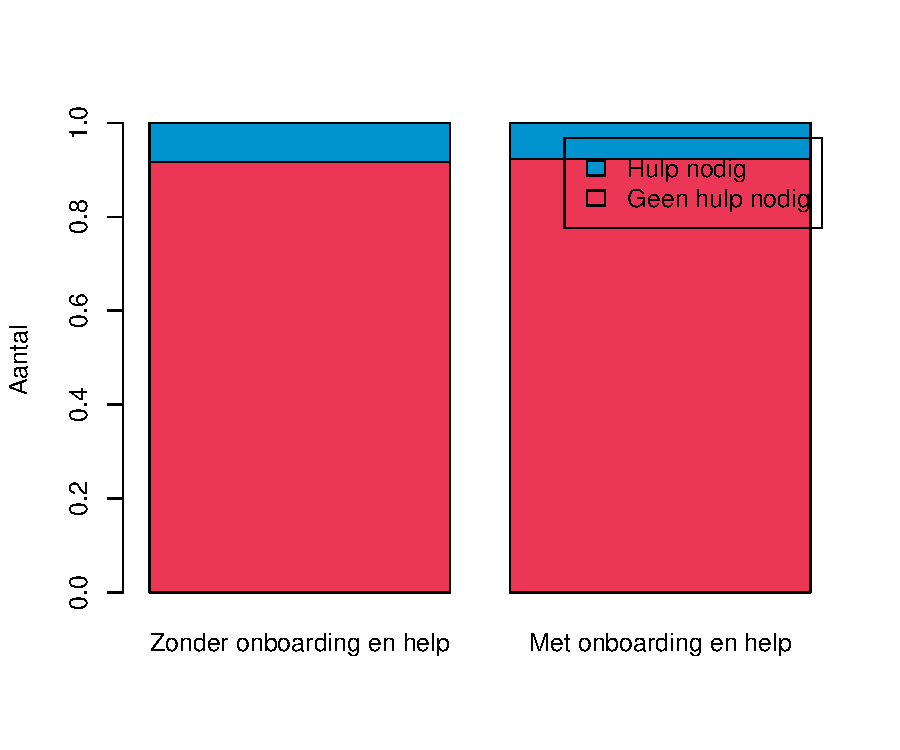
\includegraphics[width=.46\columnwidth]{beschrijving-hulp-groot-bedrag-toevoegen}}
    \caption{Had de participant hulp nodig bij het voltooien van de opdrachten?}
    \label{fig:beschrijving-hulp}
\end{figure}

Uit figuur~\ref{fig:beschrijving-hulp} kan men afleiden dat er slechts voor sommige opdrachten hulp gevraagd werd. De andere opdrachten waren voor alle participanten duidelijk, ongeacht de groep waarin ze zich bevonden.

\section{Gebruik van de voorziene functionaliteiten}
\label{sec:gebruik-functionaliteiten}

Men kan op verschillende manieren een bedrag toevoegen aan een spaardoel (figuur~\ref{fig:piggy:add-amount}). De snelste manier is door een slider te verschuiven tot het bedrag correct is en dan op de grote knop ``Add money'' te drukken. Deze slider gaat slechts tot een maximum van 50. Wanneer de gebruiker een hoger bedrag wil toevoegen moet deze op de knop met het ``+''-symbool drukken. Dit werd uitgelegd in de rondleiding doorheen de applicatie.

\begin{figure}[h!]
    \centering
    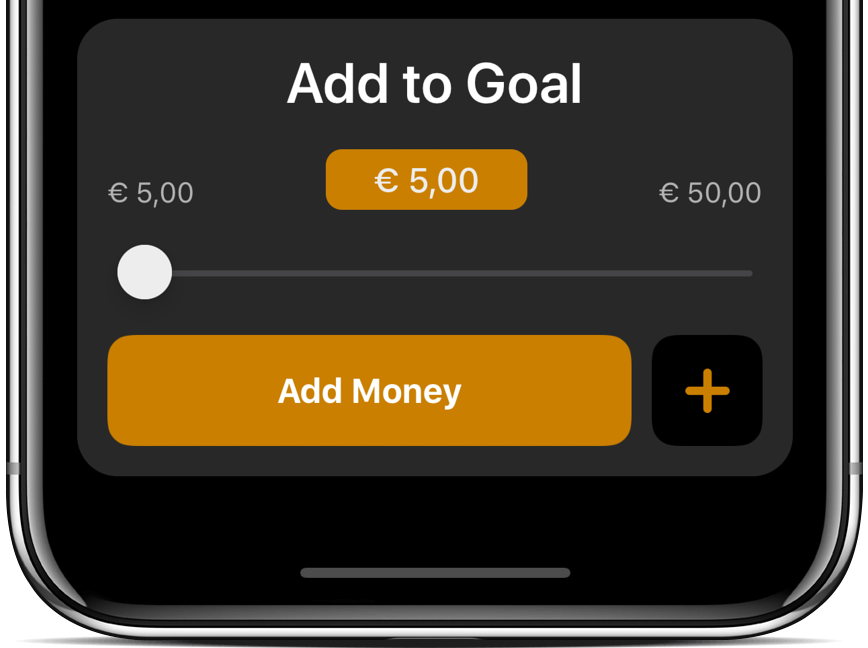
\includegraphics[width=.5\columnwidth]{piggy-add-amount}
    \caption{Verschillende manieren om een bedrag aan een spaardoel toe te voegen}
    \label{fig:piggy:add-amount}
\end{figure}

In figuur~\ref{fig:beschrijving-plus} wordt procentueel weergegeven hoeveel participanten gebruik hebben gemaakt van het ``+''-symbool bij de opdrachten die vereisten om een bedrag toe te voegen.

\begin{figure}[h]
    \centering
    \subfloat[Bedrag toevoegen]{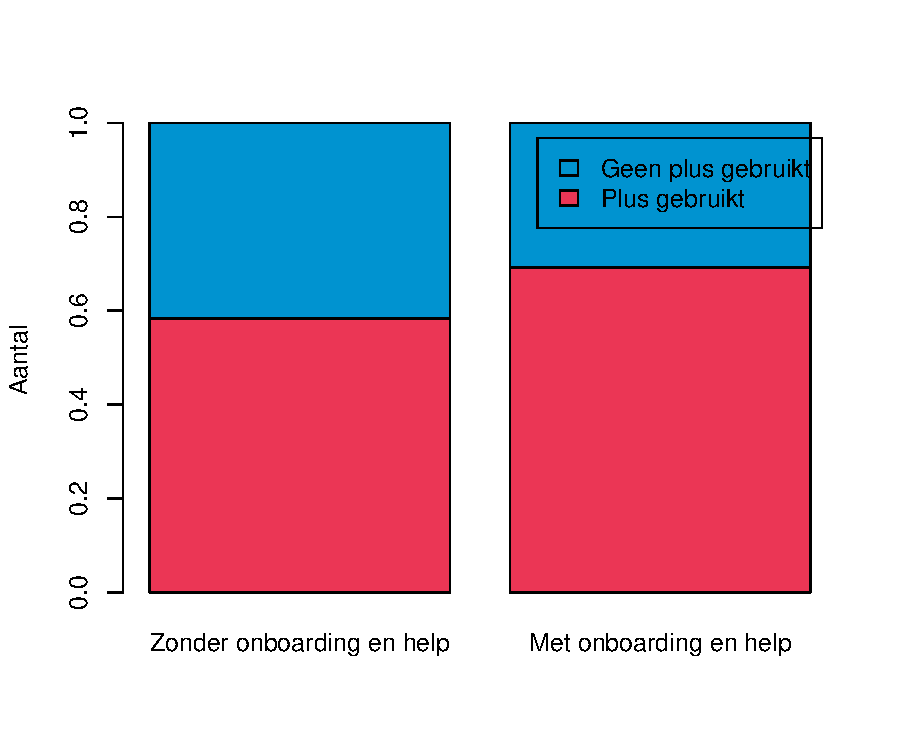
\includegraphics[width=.46\columnwidth]{beschrijving-plus-bedrag-toevoegen}}
    \qquad
    \subfloat[Groot bedrag toevoegen]{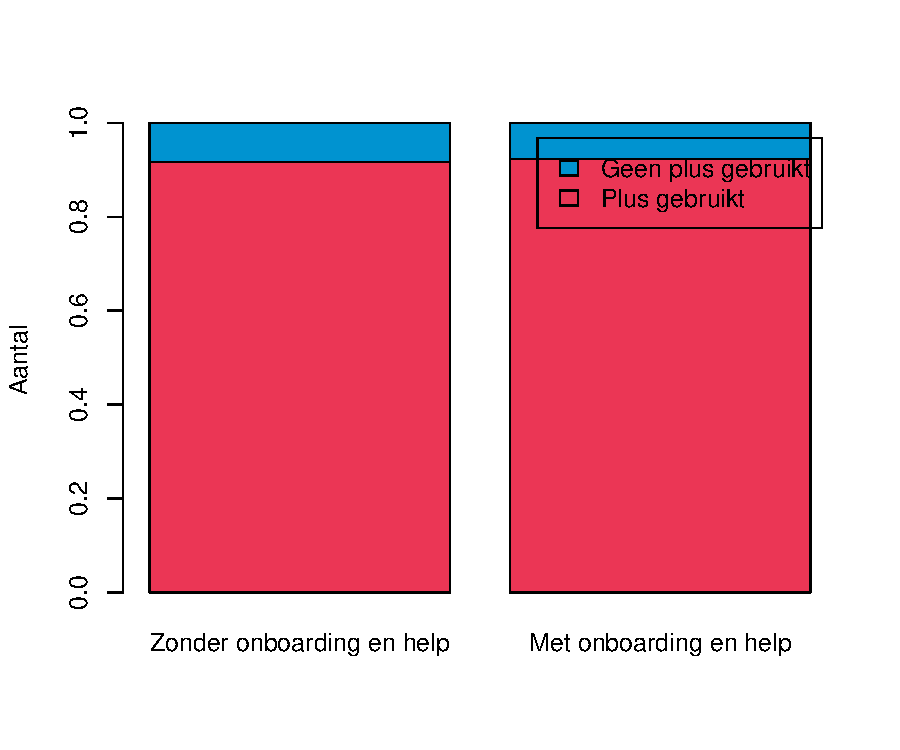
\includegraphics[width=.46\columnwidth]{beschrijving-plus-groot-bedrag-toevoegen}}
    \caption{Of de participant het ``+''-symbool gebruikt bij het toevoegen van een bedrag}
    \label{fig:beschrijving-plus}
\end{figure}

\section{De SUS-score}
\label{sec:sus}

Aan iedere participant werd gevraagd om de SUS-vragenlijst in te vullen (bijlage~\ref{bijlage:sus}). De gemiddelde resultaten hiervan worden weergegeven in tabel~\ref{tab:beschrijving-sus}. Hier kan men waarnemen dat het eventuele verschil in SUS-score zich tot een minimum zal beperken.

\begin{table}[h]
	\centering
	\begin{tabular}{r|ccccccc}
		& $Min$ & $Q_1$ & $Mdn$ & $M$ & $SD$ & $Q_3$ & $Max$ \\ \hline
		Zonder & 62.50 & 71.25 & 78.75 & 78.54 & 10.08 & 85.00 & 92.50 \\
		Met & 57.50 & 62.50 & 85.00 & 78.65 & 16.13 & 95.00 & 100.00
	\end{tabular}
	\caption{Beschrijving van de SUS-score zonder of met learnability-elementen}
	\label{tab:beschrijving-sus}
\end{table}

Zoals vermeld in hoofdstuk~\ref{sec:usability-testing:sus} bevat de SUS-vragenlijst enkele vragen die testen op learnability in plaats van op usability. Het gaat hier om vraag 4 (\textit{Ik denk dat ik de steun van een technisch persoon nodig heb om dit systeem te kunnen gebruiken}) en vraag 10 (\textit{Ik moest veel dingen leren voordat ik met dit systeem aan de slag kon}). De antwoorden op deze vragen worden visueel weergegeven in figuur~\ref{fig:beschrijving-sus}. Een beschrijving van deze antwoorden wordt weergegeven in tabellen~\ref{tab:beschrijving-sus-learnability-1} en \ref{tab:beschrijving-sus-learnability-2}. Hierbij stellen de waardes 1, 2, 3, 4 en 5 respectievelijk \textit{volledig oneens}, \textit{oneens}, \textit{neutraal}, \textit{eens} en \textit{volledig eens} voor.

\begin{figure}[h]
	\centering
	\subfloat[Zonder onboarding en help-elementen]{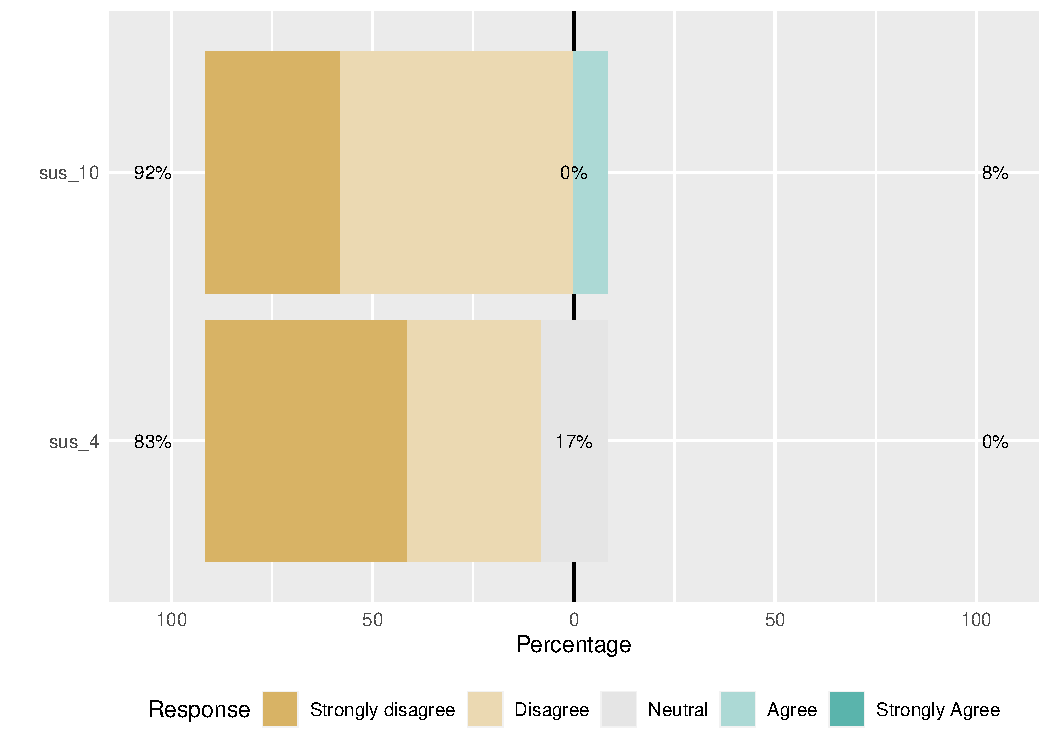
\includegraphics[width=.46\columnwidth]{beschrijving-sus-zonder}}
	\qquad
	\subfloat[Met onboarding en help-elementen]{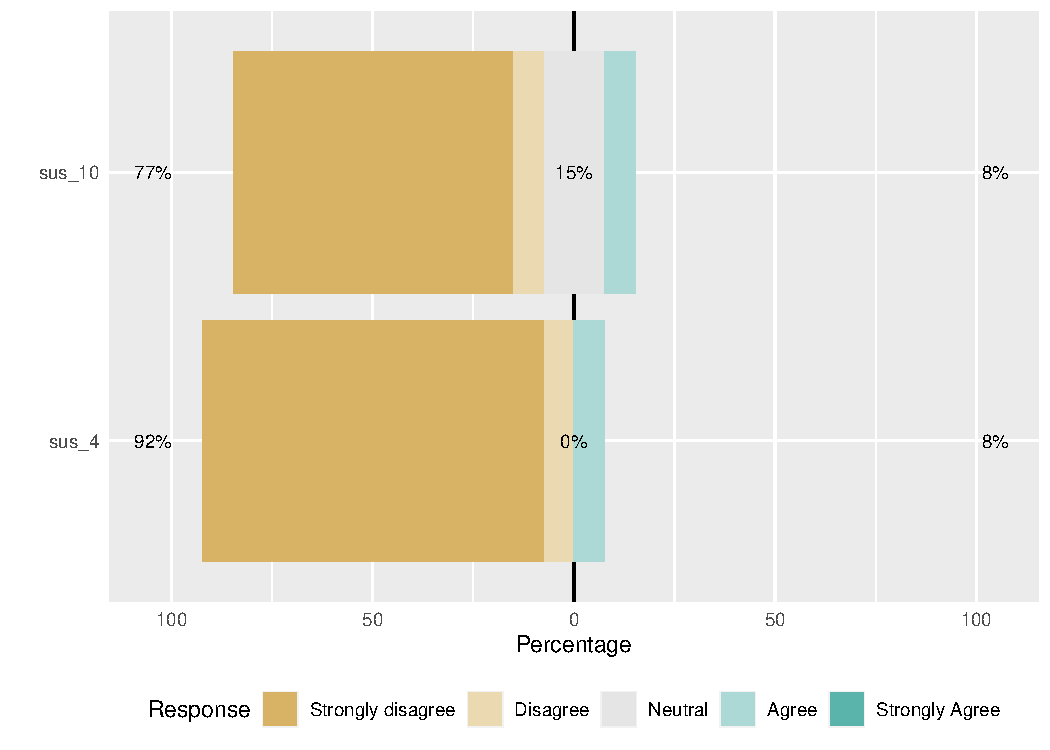
\includegraphics[width=.46\columnwidth]{beschrijving-sus-met}}
	\caption{Antwoorden op vraag 4 en 10 van de SUS-vragenlijst}
	\label{fig:beschrijving-sus}
\end{figure}

\begin{table}[h]
	\centering
	\begin{tabular}{r|ccccccc}
		& $Min$ & $Q_1$ & $Mdn$ & $M$ & $SD$ & $Q_3$ & $Max$ \\ \hline
		Vraag 4 & 1.00 & 1.00 & 1.50 & 1.67 & 0.78 & 2.00 & 3.00 \\
		Vraag 10 & 1.00 & 1.00 & 2.00 & 1.83 & 0.85 & 2.00 & 4.00
	\end{tabular}
	\caption{Beschrijving van SUS-vragen omtrent learnability zonder onboarding en help-elementen}
	\label{tab:beschrijving-sus-learnability-1}
\end{table}

\begin{table}[h]
	\centering
	\begin{tabular}{r|ccccccc}
		& $Min$ & $Q_1$ & $Mdn$ & $M$ & $SD$ & $Q_3$ & $Max$ \\ \hline
		Vraag 4 & 1.00 & 1.00 & 1.00 & 1.31 & 0.83 & 1.00 & 4.00 \\
		Vraag 10 & 1.00 & 1.00 & 1.00 & 1.62 & 1.04 & 2.00 & 4.00
	\end{tabular}
	\caption{Beschrijving van SUS-vragen omtrent learnability met onboarding en help-elementen}
	\label{tab:beschrijving-sus-learnability-2}
\end{table}

\section{Voorkeur voor onboarding en help-elementen}
\label{sec:voorkeur-onboarding}

De participanten werden na afloop gevraagd of ze de proof-of-concept applicatie liefst gebruikten indien de onboarding en help-elementen aanwezig waren. De resultaten van deze vraag worden procentueel weergegeven in figuur~\ref{fig:beschrijving-finds-better}.

\begin{figure}[h]
    \centering
    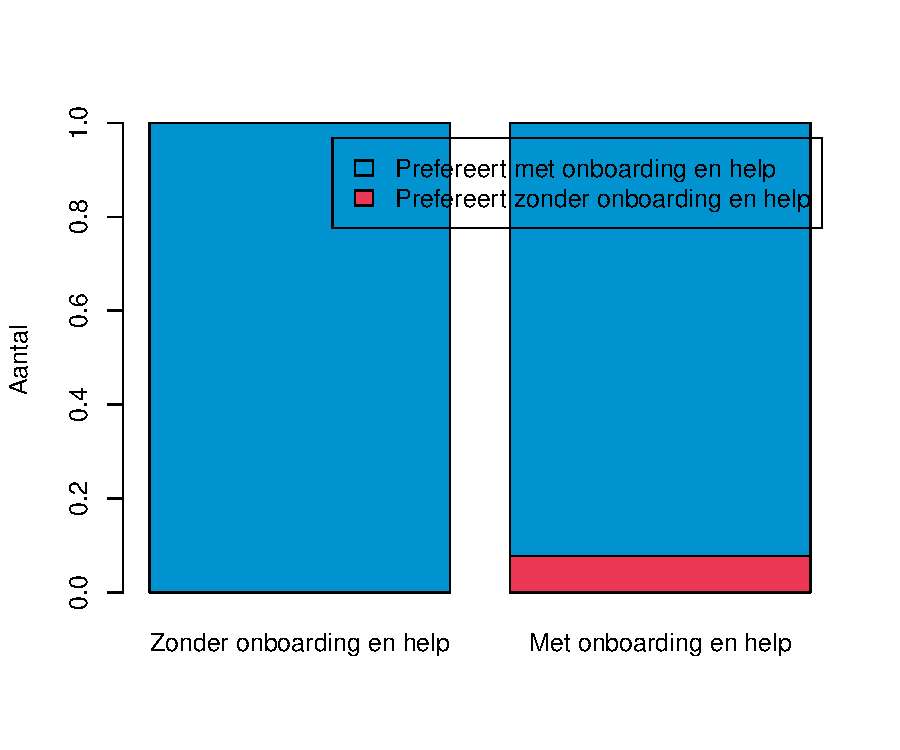
\includegraphics[width=.46\columnwidth]{beschrijving-finds-better}
    \caption{De voorkeur van de participant: een applicatie met of zonder onboarding en help-elementen}
    \label{fig:beschrijving-finds-better}
\end{figure}

Participanten die de applicatie prefereren zonder de onboarding en help-elementen maken deze keuze omdat de applicatie voor hun eenvoudig en duidelijk genoeg was. Indien de applicatie enkele meer ingewikkelde functionaliteiten zou hebben, zouden ook zij liever geholpen worden doorheen de applicatie.

\section{Voorkeur voor help-sectie}
\label{sec:voorkeur-help}

Er werd de participanten een voorbeeld getoond van de help-sectie in de applicatie (figuur~\ref{fig:piggy:help}). Hierover werd aan de participant gevraagd of deze gebruik zou maken van een gelijkaardige help-sectie in deze of andere applicaties. De resultaten van deze vraag worden procentueel weergegeven in figuur~\ref{fig:beschrijving-would-use-help}.

\begin{figure}[h]
    \centering
    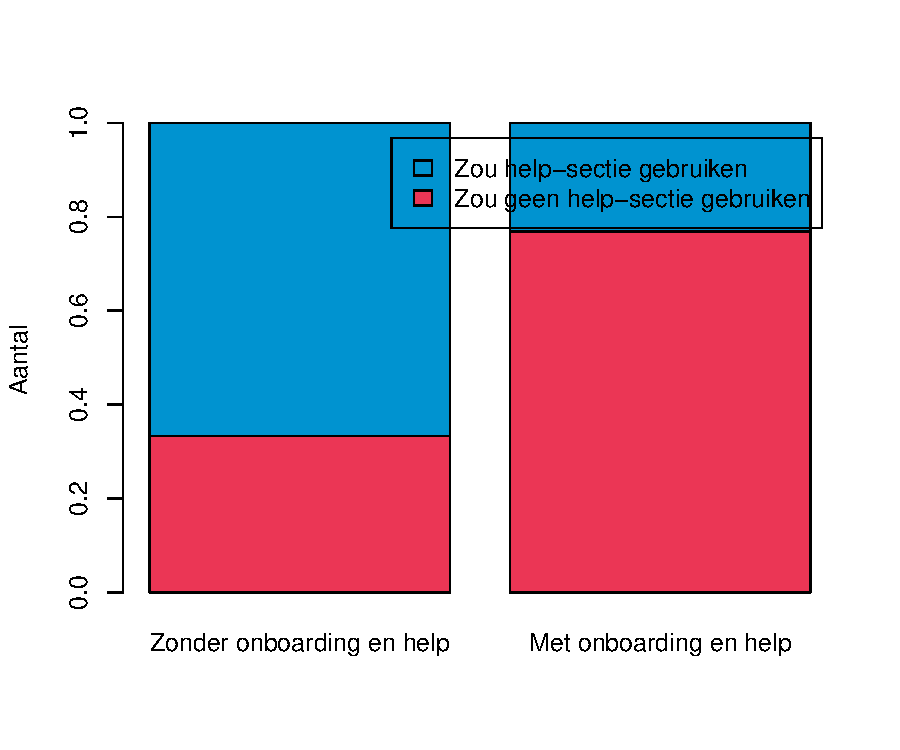
\includegraphics[width=.46\columnwidth]{beschrijving-would-use-help}
    \caption{Ziet de participant zichzelf de help-sectie gebruiken}
    \label{fig:beschrijving-would-use-help}
\end{figure}

\section{De gebruiksduur en/of levensduur van de applicatie}
\label{sec:gebruiksduur}

Om te meten of de onboarding en help-elementen al dan niet invloed hebben op de gebruiksduur en/of levensduur van de applicatie werd de participant gevraagd of deze de applicatie zou houden. Andere mogelijkheden waren dat de applicatie niet goed was, niet duidelijk was of dat men liever nog eens vergelijkt met andere beschikbare applicaties met gelijkaardige functionaliteiten. Wanneer de gebruiker voor één van deze mogelijkheden zou kiezen, zou hij of zij de applicatie dus verwijderen. De resultaten van deze vraag worden procentueel weergegeven in figuur~\ref{fig:beschrijving-would-keep}.

\begin{figure}[h]
    \centering
    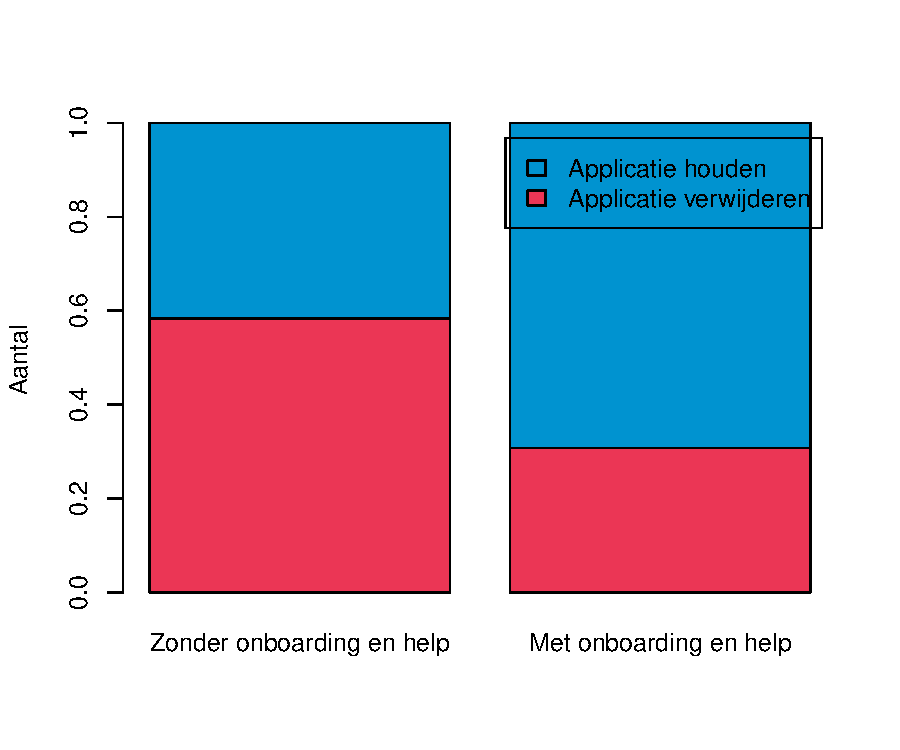
\includegraphics[width=.46\columnwidth]{beschrijving-would-keep}
    \caption{Of de participant de applicatie zou houden}
    \label{fig:beschrijving-would-keep}
\end{figure}
